\chapter{Experimental evaluation}
\label{chap:experiments}
\newcommand{\PrimaryCount}{40}
\newcommand{\PrimaryValid}{39}
\newcommand{\TimingPlanned}{120}
\newcommand{\TimingFinished}{120}
\newcommand{\TimingValid}{117}
\newcommand{\TimingResource}{3}
\newcommand{\TimingPending}{0}
\newcommand{\ContinuousMatched}{9}
\newcommand{\ContinuousEqual}{8}
\newcommand{\ContinuousExtra}{1}
\newcommand{\DiscreteEqual}{10}
\newcommand{\EqualRepair}{3}
\newcommand{\BaselineViolations}{4}
\newcommand{\ObjectiveDifferences}{0}
\newcommand{\CompleteTriples}{40}
\newcommand{\StableTriples}{40}
\newcommand{\MixedTriples}{0}
\newcommand{\GraphComparisons}{20}
\newcommand{\ActiveAvailable}{12}
\newcommand{\ActiveTwoMin}{13.55}
\newcommand{\ActiveTwoMax}{79.07}
\newcommand{\ValidIC}{10}
\newcommand{\ValidID}{10}
\newcommand{\ValidTwoF}{9}
\newcommand{\ValidThreeF}{10}

\section{Experimental questions}
We evaluate the compression and computational cost of enforcing discrete output coupling under continuous or discrete fidelity.
The primary questions are whether coupling changes the required number of vertices,
how the two fidelity definitions change compression,
and how many configuration states are discovered relative to finite construction bounds.
Computational observations are bounded by a predefined resource policy, rather than a guarantee of exhaustive completion within that policy.

The completed primary cohort and the fresh timing study are distinct evidence sets. The primary cohort has \PrimaryValid{} externally validated solutions among \PrimaryCount{} configurations. At this draft's data snapshot, \TimingFinished{} of \TimingPlanned{} scheduled fresh repetitions are recorded: \TimingValid{} validated outputs, \TimingResource{} resource exits, and \TimingPending{} pending repetitions. Pending work is not counted as a solver failure. The timing results must not be described as a completed three-repetition study while any repetitions remain pending.

\section{Datasets and preprocessing}
We use ten previously frozen pairs, comprising five protein pairs and five hurricane pairs. Table~\ref{tab:inputs} identifies every pair and its numerical thresholds. The four original pilot pairs are P1, P2, H1 and H2; the other pairs were selected before their optimization results were observed, using input-size and geometric diversity among the supplied pairs, with individual reuse discouraged where possible. The recorded selection rule used standardized size, size-imbalance, chord-to-path and relative separation features with farthest-first selection. It could not avoid the common protein anchor.

Every protein curve has 22 vertices after the existing $w=16$ subsampling of the supplied prepared curves. All five pairs share the structure/chain \texttt{1o7j.a}; previously prepared alignment to that anchor is retained. These are neither full-resolution backbone experiments nor five independent biological replicates. They cannot establish protein input-size scaling. Hurricane inputs retain all supplied track vertices, without additional subsampling, cropping or independent alignment. Coordinates remain in the common projected basin frame. Spatial coordinates alone do not establish temporal synchronization. The manifest records preparation, input hashes, provenance and reuse.
\begingroup
\small
\begin{longtable}{lllllll}
\caption{Frozen inputs and thresholds. Protein units are angstroms; hurricane units are projected kilometres. Values here are rounded to four decimals for display; the CSV and frozen configurations retain full precision.}\label{tab:inputs}\\
\toprule
ID & Pair & m & n & delta1 & delta2 & delta3 \\
\midrule
\endfirsthead
\toprule
ID & Pair & m & n & delta1 & delta2 & delta3 \\
\midrule
\endhead
P1 & 1o7j.a\_\_1d9q.d & 22 & 22 & 9.4765 & 10.1018 & 47.9645 \\
P2 & 1o7j.a\_\_1hfj.c & 22 & 22 & 9.4765 & 9.5379 & 0.9993 \\
P3 & 1o7j.a\_\_1qd1.b & 22 & 22 & 9.4765 & 10.8908 & 35.9790 \\
P4 & 1o7j.a\_\_4eca.d & 22 & 22 & 9.4765 & 8.7810 & 15.3640 \\
P5 & 1o7j.a\_\_1toh.a & 22 & 22 & 9.4765 & 10.3463 & 37.1285 \\
H1 & AL031854\_\_AL011991 & 25 & 25 & 85.2760 & 82.0160 & 426.1842 \\
H2 & EP021949\_\_EP031949 & 25 & 25 & 40.2551 & 36.4816 & 565.3421 \\
H3 & EP111954\_\_EP021984 & 25 & 82 & 62.5912 & 21.5882 & 411.7454 \\
H4 & AL072006\_\_AL011900 & 62 & 81 & 83.4081 & 81.1585 & 2969.7846 \\
H5 & EP012014\_\_EP212006 & 30 & 29 & 22.0881 & 20.7734 & 628.8969 \\
\bottomrule
\end{longtable}
\endgroup


\section{Compared methods and their constraints}
Let $A=(a_1,\ldots,a_m)$ and $B=(b_1,\ldots,b_n)$ denote the saved polygonal input curves. Outputs $A'$ and $B'$ are strictly ordered subsequences of original vertices, with both endpoints preserved. Define $k_A=|A'|$, $k_B=|B'|$, and the objective $k=\max(k_A,k_B)$. Unequal output lengths are allowed. A discrete coupling may repeat an index. Let $d_F$ denote continuous Fr\'echet distance and $d_{dF}$ discrete Fr\'echet distance, using the manuscript's notation~\cite{manuscript}.
\begin{itemize}
\item Independent continuous (IC) optimizes the two curves independently under $d_F(A,A')\leq\delta_1$ and $d_F(B,B')\leq\delta_2$.
\item Independent discrete (ID) uses $d_{dF}(A,A')\leq\delta_1$ and $d_{dF}(B,B')\leq\delta_2$ instead.
\item CPS-2F imposes the continuous fidelity constraints and $d_{dF}(A',B')\leq\delta_3$.
\item CPS-3F imposes the discrete fidelity constraints and the same discrete output-coupling constraint.
\end{itemize}
The independently optimal vertex counts minimize their maximum in the uncoupled problem. Their outputs need not satisfy $\delta_3$, and a coupling violation is not a baseline failure. Comparing CPS-2F with IC isolates the additional coupling requirement under continuous fidelity; comparing CPS-3F with ID gives the discrete counterpart. Comparing the two CPS methods changes the feasible set. Shorter CPS-2F outputs reflect its weaker continuous fidelity constraint, not superiority on an identical optimization problem. No local shortcut predicate replaces global continuous fidelity.

\section{Thresholds, resources, implementation and timing}
For each saved curve, $s_A$ and $s_B$ are its respective mean edge lengths. We use $\alpha=0.5$, $\delta_1=\alpha s_A$, $\delta_2=\alpha s_B$, and $\delta_3=d_{dF}(A,B)$ computed on the saved inputs without physical-unit rounding. Alpha was selected using earlier pilot evidence, not an independent held-out selection. The original curves are a feasible joint solution at these thresholds; a resource exit does not establish infeasibility.

All methods share a 60-second external solver allowance and a 512-MiB sampled process-tree RSS cap. CPS uses a 55-second internal soft limit, 100,000 configuration states, 20,000,000 candidate transition checks and 800,000 main single-curve edges. The edge cap applies during edge enumeration before anchored pruning; the reported completed-graph edge count is the post-pruning outgoing-entry count including waits. Independent discrete and the independent preprocessing within CPS-3F retain the existing 2,000,000-edge default per curve. Independent continuous has no analogous configuration-state or transition limit. Thus shared external limits coexist with method-specific internal work limits. The soft CPS time check is not an inner-transition-loop interrupt; the external supervisor is the backstop. These practical budgets are not theoretical sufficiency guarantees.

Separate budgets are retained for startup (60 s), input loading (15 s), warm-up (120 s), checkpointing (5 s), external validation (30 s), optional measurements (30 s), and reporting (10 s). The solver clock excludes explicit warm-up and external validation but includes any checks performed internally before return; no estimated overhead is subtracted. The continuous predicate's tolerance and numerical epsilon remain $10^{-10}$ and $10^{-9}$ respectively, with all other implementation tolerances unchanged and code hashes recorded.

The timing schedule fixes three rounds of every configuration and rotates method order across rounds while preserving pair order. Exactly one worker runs at a time. Each fresh process uses the same interpreter, thread settings (one OpenBLAS and OMP thread), isolated output-local cache policy and relevant-path warm-up. Existing process-aware readiness sampling precedes each four-method pair/round block and every resume; active workers are checked before every attempt. Readiness is outside measured phases. Pauses and timestamps remain in the progress history. No original observation is counted as a new repetition, and resource exits are not replaced by additional attempts.

Both certificate shortcuts are disabled with \texttt{certificate=False}. The implementation still computes its independent preprocessing inside the CPS solver, and that cost remains in solver time; it cannot bypass graph execution. No greedy preprocessing, alternative-subsequence search, vertex replacement or reference-guided pruning is used. Successful CPS records require explicit configuration-graph route evidence and raw status \texttt{optimal\_configuration\_graph}. Raw selected indices and counters are atomically saved before external validation. Validation checks original-vertex membership, bounds, strict order, endpoints, vertex counts, objective consistency, the applicable fidelity predicate and CPS output coupling. Optional achieved-distance searches occur afterwards. Feasibility validation alone does not independently prove optimality: optimality remains the algorithm's claim, supported separately by existing exhaustive small-instance correctness checks, not by the measured output's feasibility alone.

\section{Completion and computational performance}
Table~\ref{tab:completion} and Figure~\ref{fig:completion} retain explicit denominators. In the original cohort, IC, ID, CPS-2F and CPS-3F validated \ValidIC{}, \ValidID{}, \ValidTwoF{} and \ValidThreeF{} configurations respectively, each out of ten. The one original missing CPS-2F output is H4 (\texttt{AL072006\_\_AL011900}), which reached the transition budget after completing its single-curve graphs. Its reported work counts are observations before termination, not a completed product-graph size. Resource-limited solver times are time to termination, not time to a successful solution.
\begingroup
\small
\begin{longtable}{llllll}
\caption{Validated coverage and resource exits, keeping the original cohort separate from fresh repetitions. Pending is not a failure.}\label{tab:completion}\\
\toprule
Cohort & Method & Planned & Validated & Resource & Pending \\
\midrule
\endfirsthead
\toprule
Cohort & Method & Planned & Validated & Resource & Pending \\
\midrule
\endhead
Original & IC & 10 & 10 & 0 & 0 \\
Original & ID & 10 & 10 & 0 & 0 \\
Original & CPS-2F & 10 & 9 & 1 & 0 \\
Original & CPS-3F & 10 & 10 & 0 & 0 \\
Timing & IC & 30 & 30 & 0 & 0 \\
Timing & ID & 30 & 30 & 0 & 0 \\
Timing & CPS-2F & 30 & 27 & 3 & 0 \\
Timing & CPS-3F & 30 & 30 & 0 & 0 \\
\bottomrule
\end{longtable}
\endgroup

\begin{figure}[p]
\centering

\includegraphics[width=\textwidth]{figures/completion.pdf}
\caption{What completed under the fixed resource policy? Original configurations and fresh scheduled repetitions have separate denominators. Green means a saved output passed external feasibility validation; orange denotes resource termination, never mathematical infeasibility. Pending repetitions have no measured outcome. Exact termination reasons are retained in timing\_observations.csv and the completion table.}
\label{fig:completion}
\end{figure}
Figure~\ref{fig:timing_stability} displays individual fresh repetitions, with medians and ranges computed only from validated successes. Table~\ref{tab:timing} exposes all scheduled outcomes and the successful count for each statistic. Among \CompleteTriples{} configurations with all repetitions recorded, \StableTriples{} have the same outcome in every round and \MixedTriples{} have mixed outcomes. Across the recorded repetitions, \ObjectiveDifferences{} unexpected objective differences were detected relative to the saved primary results or other validated repetitions. This statement applies only to recorded outputs; missing repetitions cannot support a stability conclusion. Different selected subsequences can be legitimate alternative optima.
\begin{figure}[p]
\centering
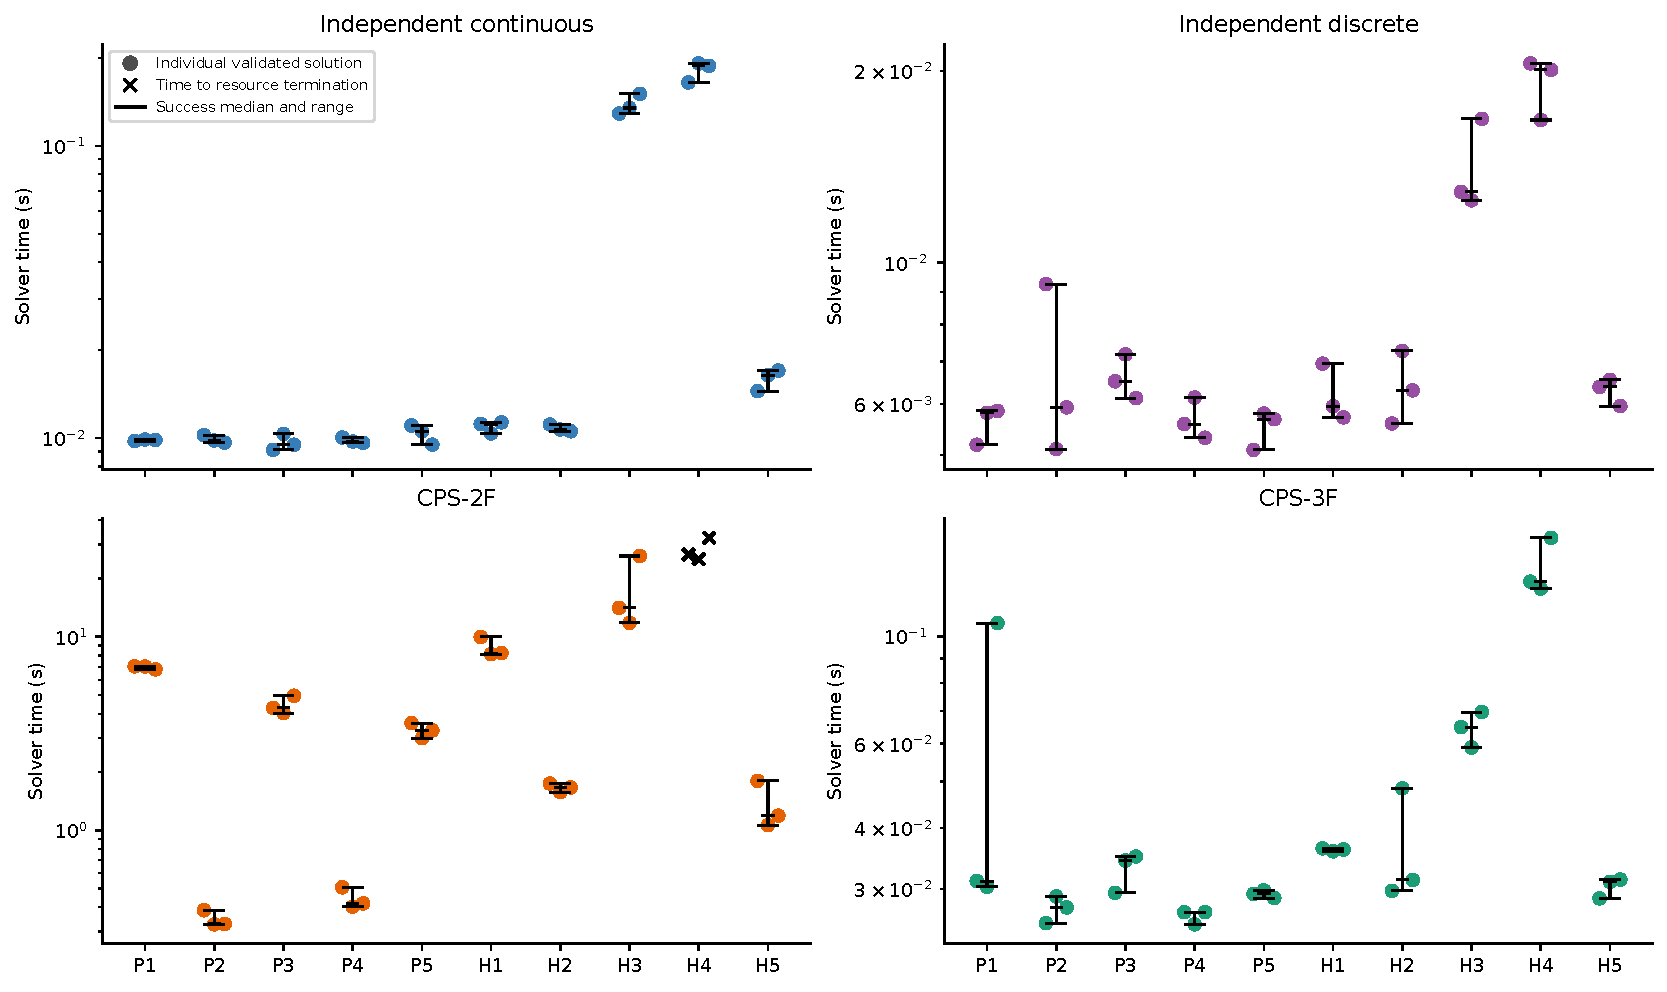
\includegraphics[width=\textwidth]{figures/timing_stability.pdf}
\caption{How stable are repeated outcomes and solver times? Each point is one scheduled fresh repetition, offset by round. Bars show median and min–max only among validated successes, with counts and all outcomes in timing\_summary.csv. Crosses are time to resource termination and are excluded from success statistics. Blank locations are unexecuted. Solver time retains internal checks; warm-up and external validation are separate. Repetitions are not independent input instances.}
\label{fig:timing_stability}
\end{figure}
Figure~\ref{fig:compression_cost} separates the quality--time observations from resource exits with unknown output quality. Figure~\ref{fig:work_indicators} relates time to recorded input size, discovered states and transition checks without fitting a scaling law. The input families and computational quantities are too restricted to infer general asymptotic behavior. Sampled memory and phase times appear in the supplement; sampled process-tree RSS includes runtime and compilation overhead and can miss unsampled peaks.
\begin{figure}[p]
\centering
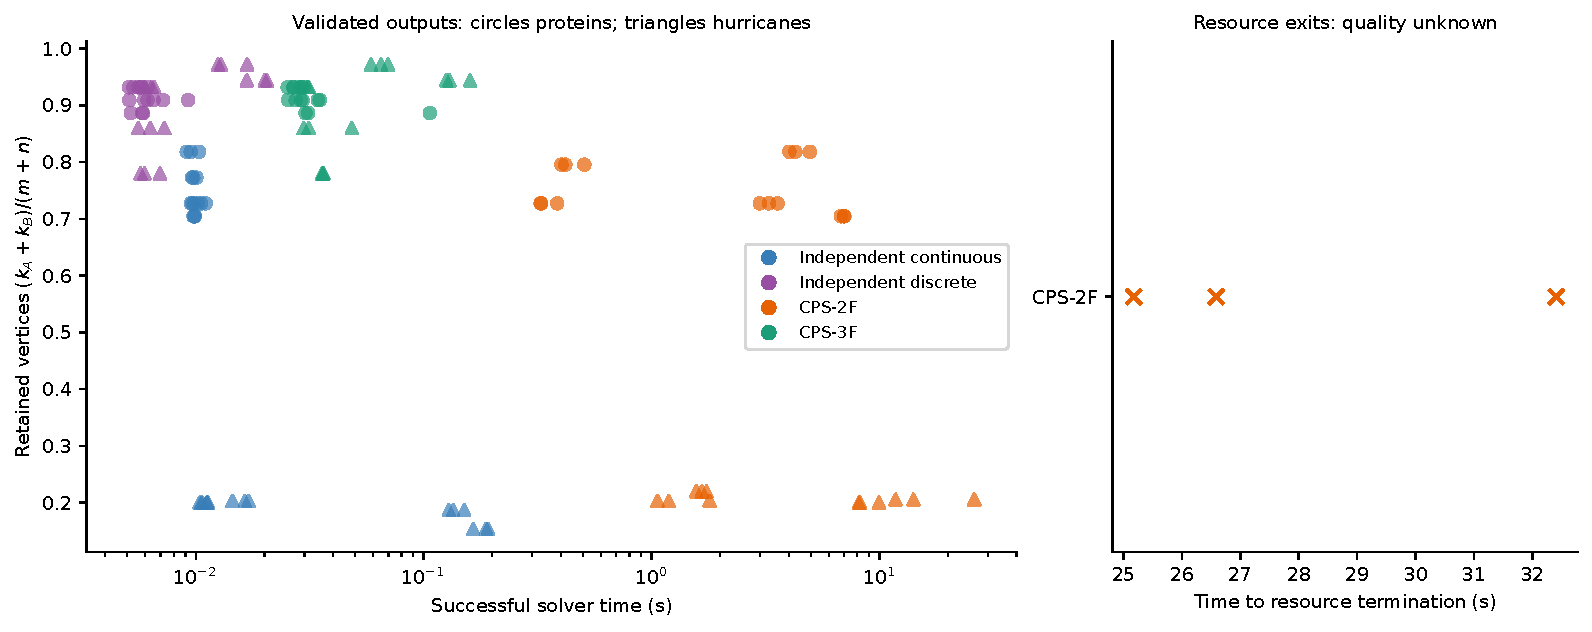
\includegraphics[width=\textwidth]{figures/compression_cost.pdf}
\caption{What compression is obtained at the observed computational cost? Only validated fresh repetitions appear in the quality panel. Protein and hurricane markers differ; colors identify methods. Continuous fidelity and discrete fidelity define different feasible sets, so shorter CPS-2F outputs do not establish superiority for an identical optimization problem. Resource exits appear separately because no solution quality is available. No historical runtime is pooled into this timing plot.}
\label{fig:compression_cost}
\end{figure}
\begin{figure}[p]
\centering
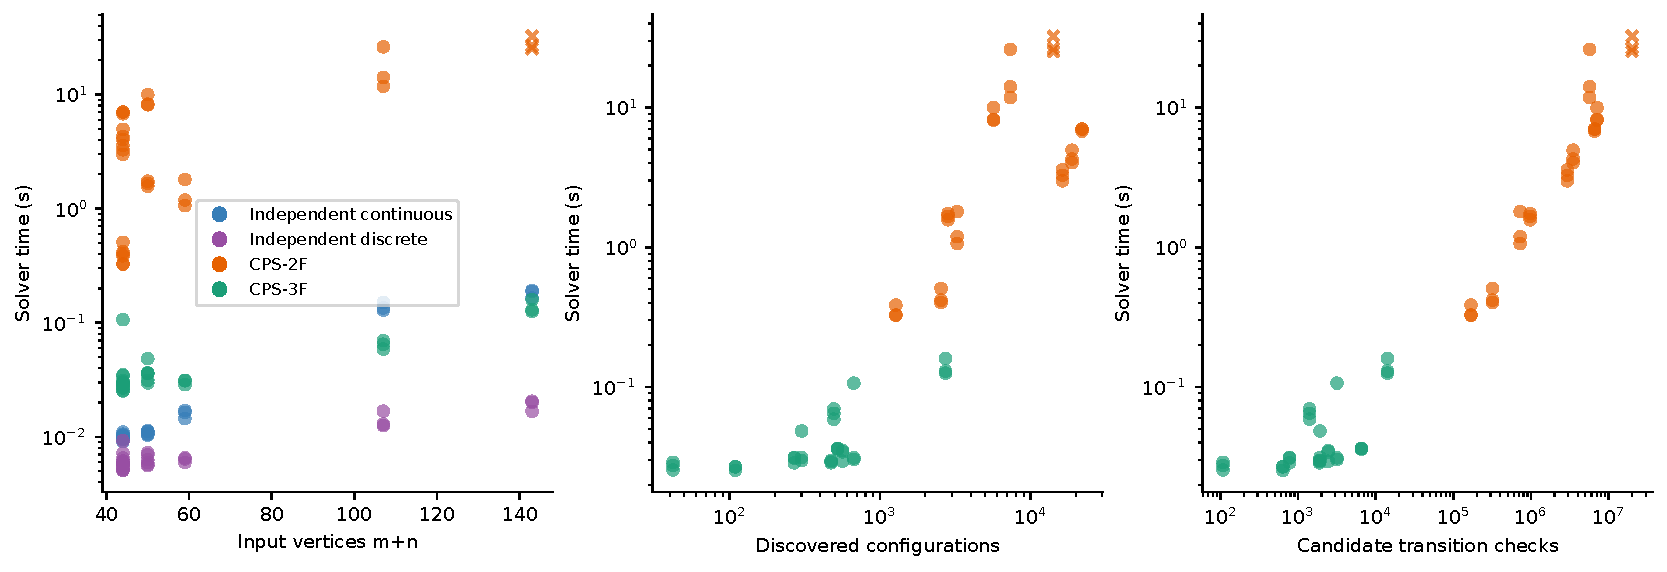
\includegraphics[width=\textwidth]{figures/work_indicators.pdf}
\caption{Which recorded work indicators accompany solver time? Fresh repetitions only; circles are validated successes and crosses are recorded unsuccessful terminations. Historical missing counters are not filled. Discovered states are not all valid states; transition checks are not unique graph edges or all machine operations. These are descriptive associations with no complexity-law fit. All protein inputs have the same sizes and share one structure.}
\label{fig:work_indicators}
\end{figure}

\section{Simplification quality and the effect of coupling}
The original cohort supplies \ContinuousMatched{} matched validated continuous-fidelity comparisons. CPS-2F and IC have equal $k$ on \ContinuousEqual{} of these, while \ContinuousExtra{} requires an additional vertex in the maximum output length. All \DiscreteEqual{} discrete-fidelity comparisons have equal CPS-3F and ID objectives. This null vertex-cost result is retained, rather than selecting only cases with a difference. The continuous independent outputs violate coupling in \BaselineViolations{} cases, and \EqualRepair{} matched cases restore coupling with unchanged $k$. Figure~\ref{fig:coupling_vertex_cost} shows both the normalized coupling and the matched-fidelity vertex cost. These counts describe this selected cohort, not a general guarantee that coupling is free.
\begin{figure}[p]
\centering
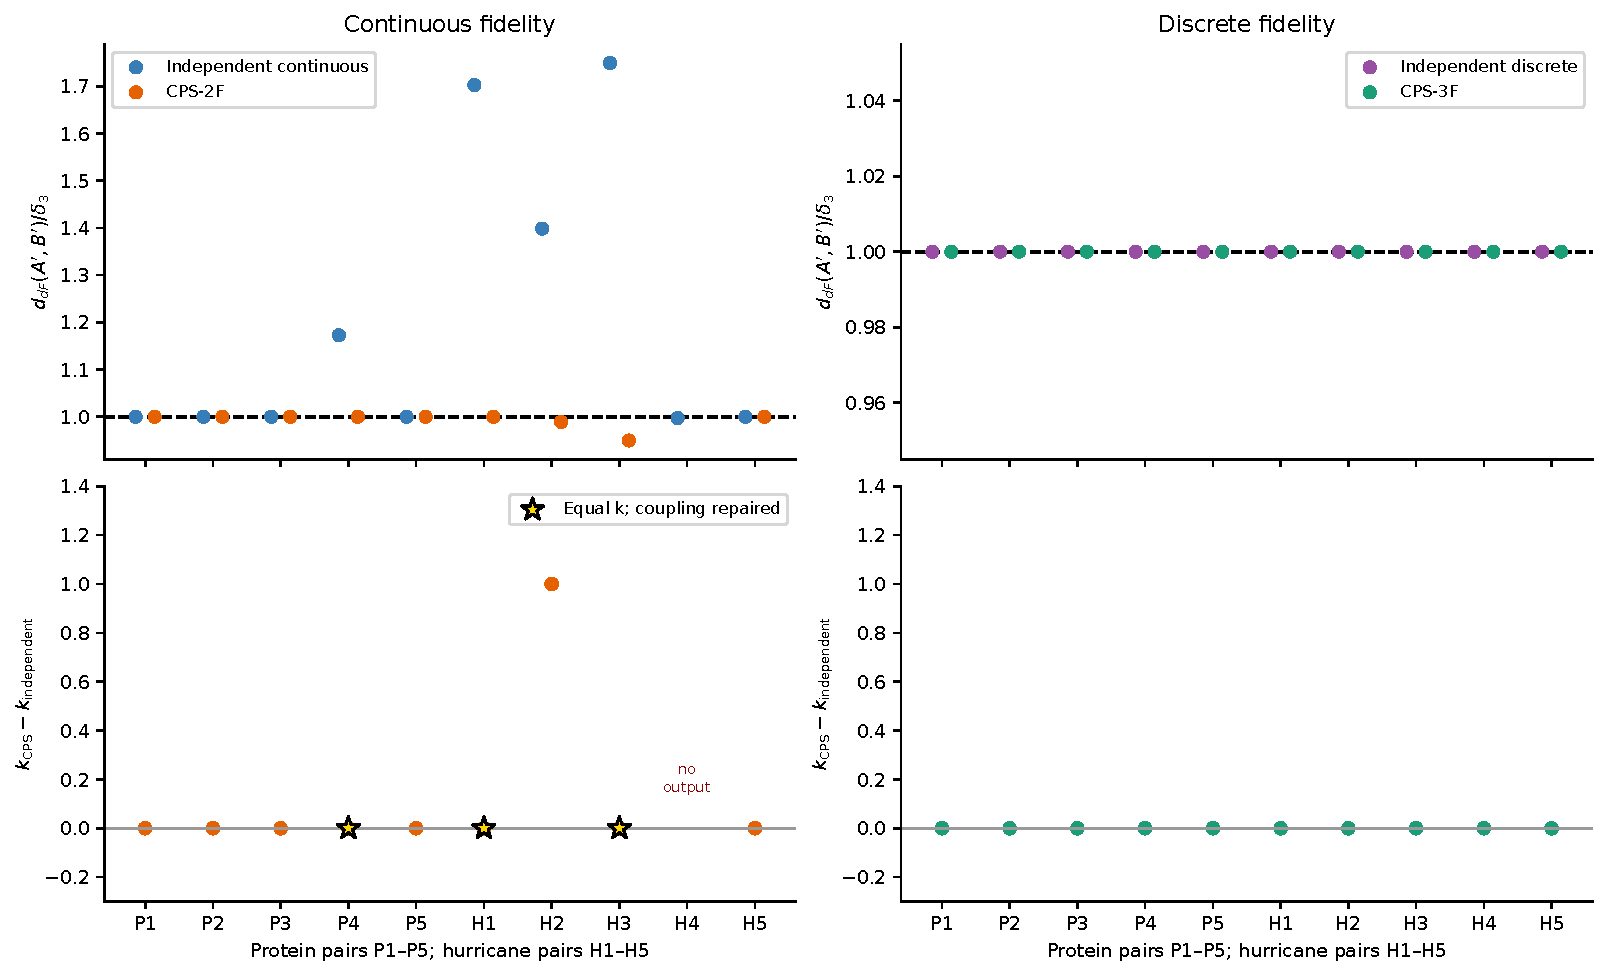
\includegraphics[width=\textwidth]{figures/coupling_vertex_cost.pdf}
\caption{Does enforcing coupling require more vertices? Original alpha=0.5 cohort: output discrete coupling divided by the shared threshold (top), and matched-fidelity objective difference (bottom). Dashed line is the coupling bound. A violation is permitted for independent baselines. Stars identify equal-objective coupling repairs. The missing CPS-2F output is a resource exit, not zero cost. Pair aliases and exact thresholds are in the input table.}
\label{fig:coupling_vertex_cost}
\end{figure}
Figure~\ref{fig:geometric_examples} uses explicitly illustrative selections. The Atlantic example demonstrates that equal $k$ does not imply equal coupling feasibility. The second hurricane example illustrates the compression difference induced by continuous versus discrete fidelity. Neither is a representative average. The reported retained-vertex fraction is $(k_A+k_B)/(m+n)$; separate output sizes remain in Table~\ref{tab:quality}.
\begin{figure}[p]
\centering
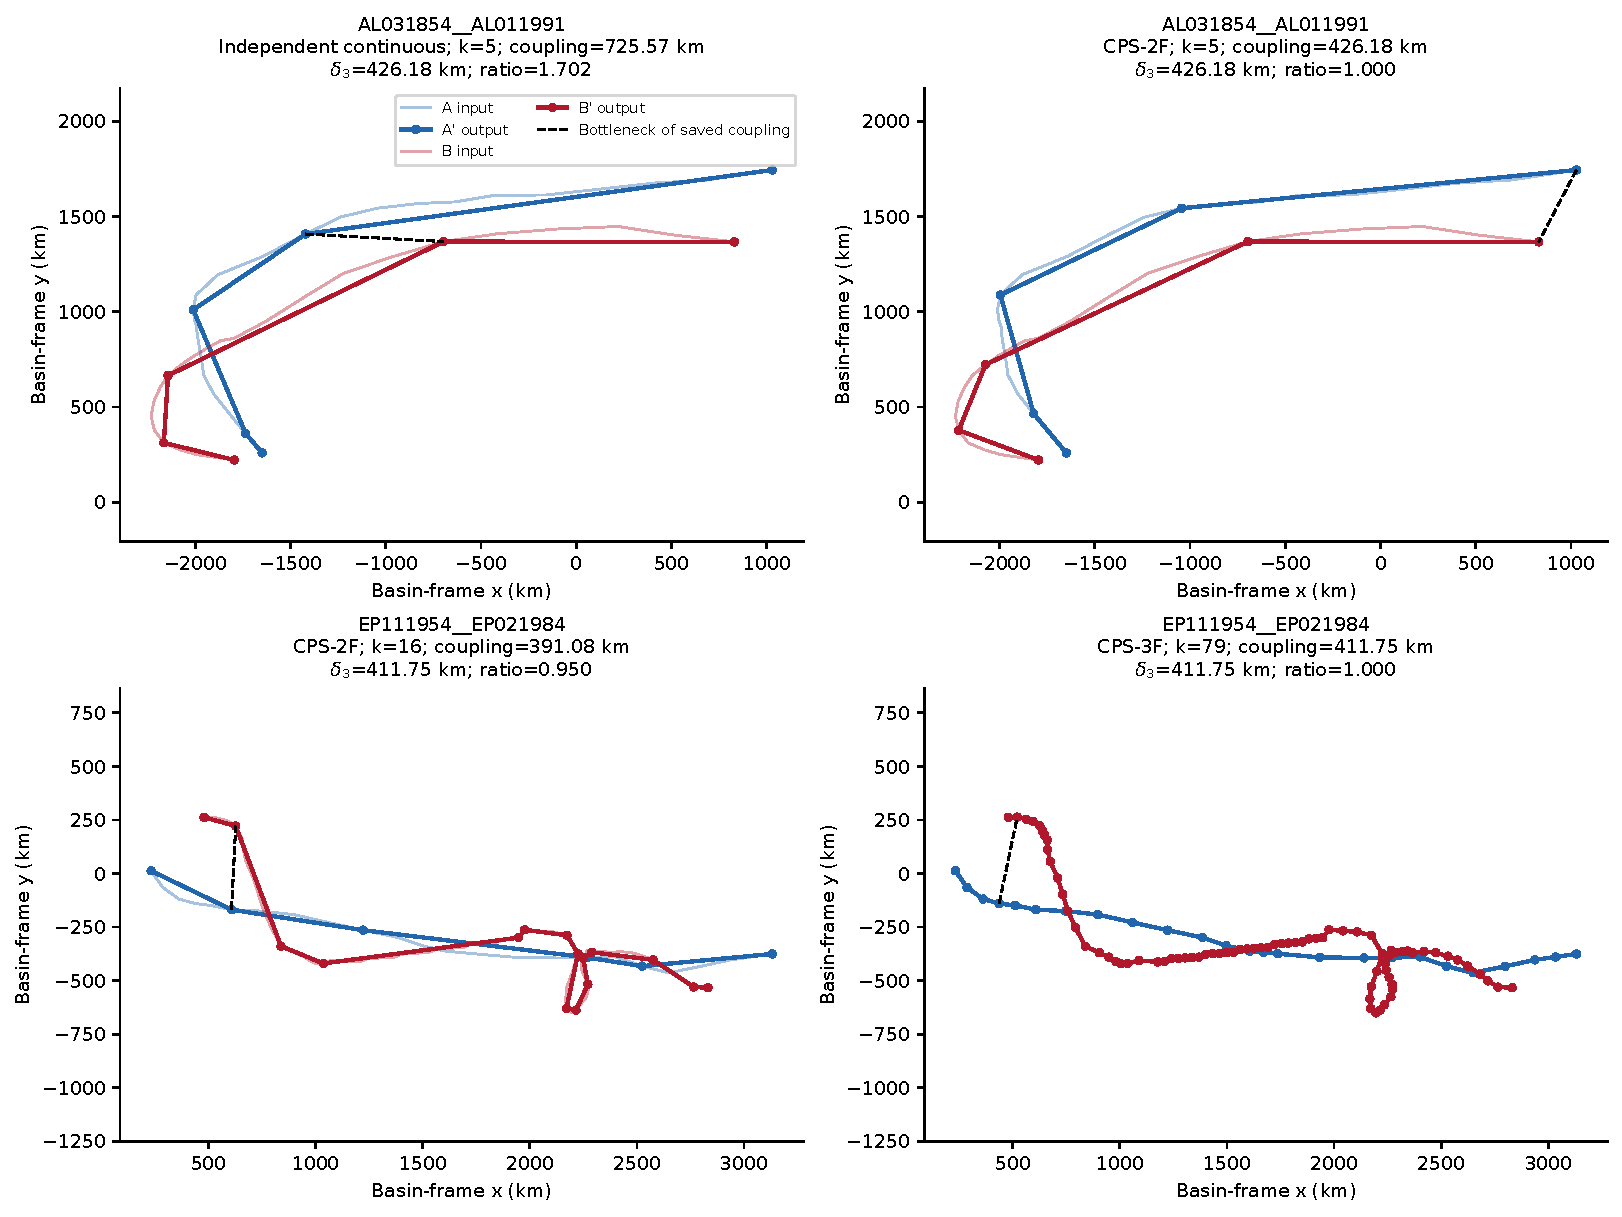
\includegraphics[width=\textwidth]{figures/geometric_examples.pdf}
\caption{Illustrative selections, not representative averages. Top: Atlantic AL031854/AL011991 has equal k=5 for independent continuous and CPS-2F, but only the coupled output satisfies the coupling bound. Bottom: EP111954/EP021984 has CPS-2F k=16 and CPS-3F k=79, illustrating the change in feasible set between continuous and discrete fidelity. Pale curves are supplied inputs; strong curves and markers are selected original vertices. The dashed segment marks a bottleneck pair in the saved discrete coupling. Distances are rounded for display only; full-precision saved thresholds are unchanged. No independent storm alignment or temporal synchronization is inferred.}
\label{fig:geometric_examples}
\end{figure}

\section{Observed graph size relative to finite bounds}
For a nondegenerate curve with $m$ original vertices, each sphere around an original vertex intersects each straight edge in at most two locations. The construction assumes no edge is contained in a sphere boundary; the implementation skips degenerate edges and retains original endpoints. Thus the number of added matching locations satisfies $a_A\leq 2m(m-1)$, and similarly $a_B\leq 2n(n-1)$~\cite[Observation 4, printed p.~18 (PDF p.~26)]{thesis}. Counts refer to distinct interior curve parameters after tolerance-based merging, not distinct spatial coordinates. Auxiliary matching locations are not selectable output vertices.

Single-curve dense index spaces have sizes $S_A=m(m+a_A)$ and $S_B=n(n+a_B)$. Anchored reachability pruning leaves $H_A$ and $H_B$ active vertices, including source and terminal. A product configuration chooses one vertex from each graph, giving the finite bounds
\begin{align}
B_{\mathrm{input}}^{2F}&=mn\,[m+2m(m-1)]\,[n+2n(n-1)],\\
B_{\mathrm{extended}}^{2F}&=mn(m+a_A)(n+a_B),\\
B_{\mathrm{active}}&=H_AH_B.
\end{align}
For CPS-3F there are no auxiliary locations and $B_{\mathrm{input}}^{3F}=m^2n^2$. Source and terminal require no additional states outside these products. These are combinatorial counts from the construction, not evaluations of an $O(\cdot)$ expression with an assumed constant of one. The theoretical CPS-2F $O(m^3n^3)$ expression counts potential configurations; see the thesis section 5.1, printed p.~26 (PDF p.~34), and manuscript section 4.4, PDF pp.~15--16~\cite{thesis,manuscript}.

Let $D$ be the number of discovered configurations, including the source. Figure~\ref{fig:graph_size_levels} compares $D$, $H_AH_B$, and $B_{\mathrm{input}}$ and names the denominator for each percentage. Active products can still include coupling-invalid states. A completed search need not enumerate all possible, valid or reachable configurations. For interrupted runs, $D$ is only observed before termination. Neither $100D/B_{\mathrm{input}}$ nor $100D/(H_AH_B)$ is an execution-progress estimate. Missing historical active-state counters remain missing and are not backfilled with measurements from timing repetitions.

Active-product bounds are available for \ActiveAvailable{} of the \GraphComparisons{} original CPS observations. Among the recorded CPS-2F active-product comparisons, discovered-state occupancy ranges from \ActiveTwoMin\% to \ActiveTwoMax\%, including the interrupted observation. These percentages describe the explored subset relative to a particular combinatorial denominator, not a universal sparsity ratio or a proof that all valid states were searched.

Single-graph edge counts include one wait self-transition per active vertex. Their finite bound is $E_A\leq H_A(H_A+1)/2$ (and analogously for B), because each non-wait edge strictly advances the topological index and entries are unique. Where both completed graphs have counters, candidate transition checks are bounded by $E_AE_B-H_AH_B$: each outgoing-entry pair defines one product transition candidate, simultaneous waits are excluded and a source is popped at most once. The implemented counter increments after the coupling filter; a budget-triggering check may be counted before relaxation. This does not establish that checks are stored unique graph edges. The product graph is implicit and no observed unique-edge count is available. Dynamic-programming labels are another quantity: at most $m$ A-hop labels per configuration in this implementation, giving a finite $mH_AH_B$ bound without an observed label count. Full formulas, assumptions and missing-data reasons are in the graph-bound table.
\begin{figure}[p]
\centering

\includegraphics[width=\textwidth]{figures/graph_size_levels.pdf}
\caption{How large is the explored state set relative to finite construction bounds? Original cohort only. D counts discovered configurations, including the source. The input-only bound follows sphere–edge intersection counting; H\_A H\_B is the product of active single-curve vertices after anchored pruning. Missing historical H counters remain missing. Crosses mark counts observed before termination. Neither completed search nor bound occupancy implies enumeration of all valid states; percentages do not measure progress. Formulas and assumptions are given in the graph-size section and graph\_bounds.csv.}
\label{fig:graph_size_levels}
\end{figure}

\section{Limitations}
The cohort is small, selected for a bounded pilot, and uses a pilot-informed alpha. Shared protein structure and identical protein sizes prevent claims of independent biological replication or protein scaling. Storm reuse and coordinate preparation are recorded; spatial coupling is not evidence of temporal correspondence. Three repeated executions of an input do not create three independent input instances or support a claim of statistical significance. Outcome variation must remain visible, and failed-run times must not enter successful-runtime averages.

Continuous and discrete fidelity are different scientific constraints. Feasibility checks do not independently certify optimality; resource exits do not certify infeasibility. External budgets are shared but internal work limits are method-specific. Historical instrumentation differs, historical missing counters remain missing, and the timing study is kept separate from original single observations. Process-aware readiness cannot guarantee an otherwise idle host throughout each measured phase. No general complexity law, exact packedness value, topological-preservation conclusion or publication-scale performance guarantee follows from these results. The provisional experimental prose in the supplied documents is not treated as measured evidence.

\section*{Supplementary saved-result tables and figure}
\begingroup
\small
\begin{longtable}{lllllll}
\caption{Fresh timing outcomes, with successful solver times only. Individual resource-exit times and all phase timings are available in timing\_observations.csv. Three repetitions were scheduled per configuration; blank statistics do not mean zero.}\label{tab:timing}\\
\toprule
Pair & Method & Valid n & R1 & R2 & R3 & Success median [min,max] s \\
\midrule
\endfirsthead
\toprule
Pair & Method & Valid n & R1 & R2 & R3 & Success median [min,max] s \\
\midrule
\endhead
H1 & IC & 3 & valid & valid & valid & 0.01117 [0.01037,0.01132] \\
H1 & ID & 3 & valid & valid & valid & 0.005956 [0.005723,0.006948] \\
H1 & CPS-2F & 3 & valid & valid & valid & 8.219 [8.126,9.98] \\
H1 & CPS-3F & 3 & valid & valid & valid & 0.03616 [0.03585,0.03636] \\
H2 & IC & 3 & valid & valid & valid & 0.0107 [0.01056,0.01113] \\
H2 & ID & 3 & valid & valid & valid & 0.006309 [0.005599,0.007275] \\
H2 & CPS-2F & 3 & valid & valid & valid & 1.664 [1.572,1.741] \\
H2 & CPS-3F & 3 & valid & valid & valid & 0.03128 [0.0297,0.04841] \\
P1 & IC & 3 & valid & valid & valid & 0.009855 [0.009765,0.009897] \\
P1 & ID & 3 & valid & valid & valid & 0.005818 [0.005185,0.005861] \\
P1 & CPS-2F & 3 & valid & valid & valid & 7.01 [6.777,7.022] \\
P1 & CPS-3F & 3 & valid & valid & valid & 0.03111 [0.03028,0.1065] \\
P2 & IC & 3 & valid & valid & valid & 0.009814 [0.009651,0.01024] \\
P2 & ID & 3 & valid & valid & valid & 0.005934 [0.005102,0.009255] \\
P2 & CPS-2F & 3 & valid & valid & valid & 0.3278 [0.3262,0.3856] \\
P2 & CPS-3F & 3 & valid & valid & valid & 0.02743 [0.02545,0.0289] \\
P3 & IC & 3 & valid & valid & valid & 0.009495 [0.009117,0.01034] \\
P3 & ID & 3 & valid & valid & valid & 0.006518 [0.006132,0.007182] \\
P3 & CPS-2F & 3 & valid & valid & valid & 4.283 [4.028,4.954] \\
P3 & CPS-3F & 3 & valid & valid & valid & 0.03432 [0.02941,0.03497] \\
P4 & IC & 3 & valid & valid & valid & 0.009739 [0.00963,0.01005] \\
P4 & ID & 3 & valid & valid & valid & 0.005585 [0.005318,0.006148] \\
P4 & CPS-2F & 3 & valid & valid & valid & 0.4185 [0.4025,0.507] \\
P4 & CPS-3F & 3 & valid & valid & valid & 0.02681 [0.0253,0.02683] \\
P5 & IC & 3 & valid & valid & valid & 0.01055 [0.0095,0.01105] \\
P5 & ID & 3 & valid & valid & valid & 0.005684 [0.00509,0.005804] \\
P5 & CPS-2F & 3 & valid & valid & valid & 3.277 [2.989,3.578] \\
P5 & CPS-3F & 3 & valid & valid & valid & 0.02927 [0.02868,0.02975] \\
H3 & IC & 3 & valid & valid & valid & 0.1348 [0.129,0.1507] \\
H3 & ID & 3 & valid & valid & valid & 0.01292 [0.01253,0.01681] \\
H3 & CPS-2F & 3 & valid & valid & valid & 14.11 [11.8,26.12] \\
H3 & CPS-3F & 3 & valid & valid & valid & 0.06484 [0.05884,0.06968] \\
H4 & IC & 3 & valid & valid & valid & 0.1879 [0.1648,0.1915] \\
H4 & ID & 3 & valid & valid & valid & 0.02006 [0.01674,0.02053] \\
H4 & CPS-2F & 0 & T-limit & T-limit & T-limit & -- \\
H4 & CPS-3F & 3 & valid & valid & valid & 0.1298 [0.1256,0.1599] \\
H5 & IC & 3 & valid & valid & valid & 0.0164 [0.01447,0.01703] \\
H5 & ID & 3 & valid & valid & valid & 0.006387 [0.00596,0.006551] \\
H5 & CPS-2F & 3 & valid & valid & valid & 1.19 [1.062,1.8] \\
H5 & CPS-3F & 3 & valid & valid & valid & 0.03099 [0.02864,0.03133] \\
\bottomrule
\end{longtable}
\endgroup

\begingroup
\small
\begin{longtable}{lllllll}
\caption{Original-cohort solution details. Independent coupling ratios above one are descriptive violations of a constraint the baseline does not enforce. Missing values correspond to no validated output.}\label{tab:quality}\\
\toprule
pair\_alias & method & kA & kB & k & retained\_total & coupling\_ratio \\
\midrule
\endfirsthead
\toprule
pair\_alias & method & kA & kB & k & retained\_total & coupling\_ratio \\
\midrule
\endhead
H1 & IC & 5 & 5 & 5 & 0.2 & 1.702 \\
H1 & ID & 20 & 19 & 20 & 0.78 & 1 \\
H1 & CPS-2F & 5 & 5 & 5 & 0.2 & 1 \\
H1 & CPS-3F & 20 & 19 & 20 & 0.78 & 1 \\
H2 & CPS-2F & 5 & 6 & 6 & 0.22 & 0.9892 \\
H2 & CPS-3F & 25 & 18 & 25 & 0.86 & 1 \\
H2 & IC & 5 & 5 & 5 & 0.2 & 1.398 \\
H2 & ID & 25 & 18 & 25 & 0.86 & 1 \\
P1 & IC & 16 & 15 & 16 & 0.7045 & 1 \\
P1 & ID & 20 & 19 & 20 & 0.8864 & 1 \\
P1 & CPS-2F & 16 & 15 & 16 & 0.7045 & 1 \\
P1 & CPS-3F & 20 & 19 & 20 & 0.8864 & 1 \\
P2 & CPS-2F & 16 & 16 & 16 & 0.7273 & 1 \\
P2 & CPS-3F & 20 & 20 & 20 & 0.9091 & 1 \\
P2 & IC & 16 & 16 & 16 & 0.7273 & 1 \\
P2 & ID & 20 & 20 & 20 & 0.9091 & 1 \\
P3 & IC & 16 & 20 & 20 & 0.8182 & 1 \\
P3 & ID & 20 & 20 & 20 & 0.9091 & 1 \\
P3 & CPS-2F & 16 & 20 & 20 & 0.8182 & 1 \\
P3 & CPS-3F & 20 & 20 & 20 & 0.9091 & 1 \\
P4 & IC & 16 & 18 & 18 & 0.7727 & 1.173 \\
P4 & ID & 20 & 21 & 21 & 0.9318 & 1 \\
P4 & CPS-2F & 17 & 18 & 18 & 0.7955 & 1 \\
P4 & CPS-3F & 20 & 21 & 21 & 0.9318 & 1 \\
P5 & IC & 16 & 16 & 16 & 0.7273 & 1 \\
P5 & ID & 20 & 21 & 21 & 0.9318 & 1 \\
P5 & CPS-2F & 16 & 16 & 16 & 0.7273 & 1 \\
P5 & CPS-3F & 20 & 21 & 21 & 0.9318 & 1 \\
H3 & IC & 4 & 16 & 16 & 0.1869 & 1.749 \\
H3 & ID & 25 & 79 & 79 & 0.972 & 1 \\
H3 & CPS-2F & 6 & 16 & 16 & 0.2056 & 0.9498 \\
H3 & CPS-3F & 25 & 79 & 79 & 0.972 & 1 \\
H4 & IC & 12 & 10 & 12 & 0.1538 & 0.9973 \\
H4 & ID & 60 & 75 & 75 & 0.9441 & 1 \\
H4 & CPS-2F & -- & -- & -- & -- & -- \\
H4 & CPS-3F & 60 & 75 & 75 & 0.9441 & 1 \\
H5 & IC & 5 & 7 & 7 & 0.2034 & 1 \\
H5 & ID & 28 & 27 & 28 & 0.9322 & 1 \\
H5 & CPS-2F & 5 & 7 & 7 & 0.2034 & 1 \\
H5 & CPS-3F & 28 & 27 & 28 & 0.9322 & 1 \\
\bottomrule
\end{longtable}
\endgroup

\begin{figure}[p]
\centering
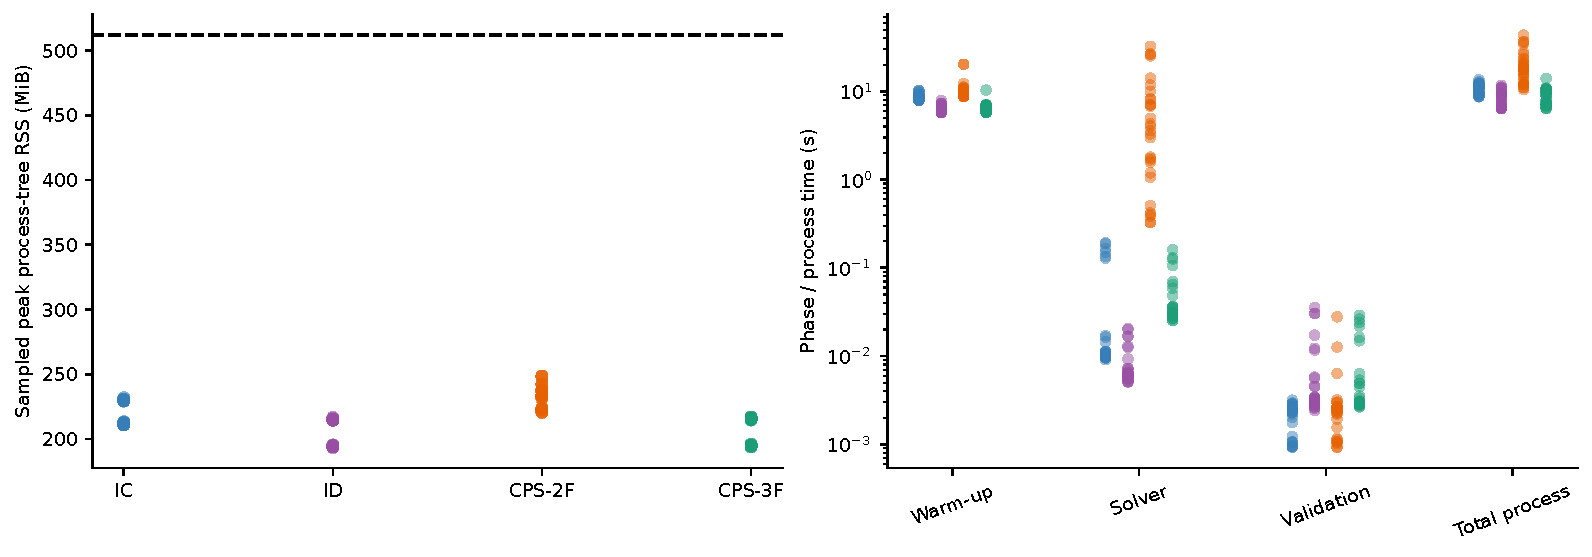
\includegraphics[width=\textwidth]{figures/supplement_memory_phases.pdf}
\caption{Supplement: sampled peak process-tree RSS and separate recorded times for fresh repetitions. Memory includes interpreter, compilation, allocator and monitoring-visible descendants, and is an approximate sampled peak, not exact algorithm memory. Phase values and unsuccessful outcomes remain individually available in the observation table; total process time is not solver time.}
\label{fig:supplement_memory_phases}
\end{figure}
\begin{thebibliography}{9}
\bibitem{thesis} G. Gozoltzani. Supplied MSc thesis, \emph{M\_Sc\_\_Thesis\_\_\_Galit\_Gozoltzani.pdf}. Construction references: Observation 4 and section 5.1. The file hash is recorded in the accompanying provenance.
\bibitem{manuscript} \emph{Chain Pair Simplification under the Continuous Fr\'echet Distance}. Supplied manuscript, sections 3.1, 4.1 and 4.4. Experimental text is provisional; the file hash is recorded in the accompanying provenance.
\end{thebibliography}
